\section{numerische Integration}

Eine Funktion durch aufteilen in Teilintervalle + Approximation angenähert
Integrieren.

\subsection{Rechteck-/Trapezregel}

Zur Approximation von Integral $$I = \int_a^b{f(x) dx}$$ durch ein Rechteck/Trapez

{\large
\begin{description}
	\item[Rechteckregel] $$Rf = f(\frac{a+b}{2}) * (b - a)$$
	\item[Trapezregel] $$Tf = \frac{f(a)+f(b)}{2} * (b - a)$$
\end{description}
}



\subsubsection{summierte Rechteck-/Trapezregel}

\begin{itemize}
	\item $f : [a, b] \to \R$ stetig
	\item $n \in \N$ Anzahl Subintervalle $[x_i, x_{i+1}]$
	\item $i \in [0, n-1]$ und $x_n = b$
	\item Subintervalle von konstanter Breite $h = x_{i+1} - x_i
		      = \frac{b-a}{n} \rarr x_i = a + i * h$
\end{itemize}

{\large
$$Rf(h) = h * \sum_{i=0}^{n-1}{f(x_i + \frac{h}{2})}$$
$$Tf(h) = h * \left(\frac{f(a) + f(b)}{2} + \sum_{i=1}^{n-1}{f(x_i)}\right)$$
}





\subsection{Simpson-Regel}

Annäherung durch ein Polynom 2. Grades anstatt Rechteck/Trapez



{\large
$$I = \int_a^b{f(x) dx}
	\approx \frac{b-a}{6} \left(f(a) + 4f(\frac{a+b}{2}) + f(b)\right)$$
}


\subsubsection{summierte Simpson-Regel}

Ausgangslage identisch zu summierte Rechteck-/Trapezregel

\begin{center}
	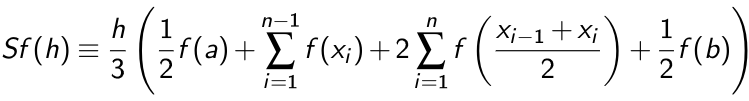
\includegraphics[scale=0.28]{int-sum-simpson}
\end{center}


Kann auch als gewichtetes Mittel von Trapez- \& Rechteckregel geschrieben werden:

$$Sf(h) = \frac{1}{3}(Tf(h) + 2Rf(h))$$




\subsection{Fehlerabschätzung der \textcolor{yellow}{summierten} Formeln
	(Rechteck/Trapez/Simpson)}
% TODO code

Die summierte Rechteckregel ist erwartungsweise doppelt so genau wie die Trapezregel,
Simpson mit Abstand am genauesten. ($h = \frac{b-a}{n}$)

{\large
		\begin{align*}
			|\int_a^b{f(x) dx} - Rf(h)| \quad \le & \quad \frac{h^2}{24} (b-a) * \max_{x \in [a, b]} |f''(x)|       \\
			|\int_a^b{f(x) dx} - Tf(h)| \quad \le & \quad \frac{h^2}{12} (b-a) * \max_{x \in [a, b]} |f''(x)|       \\
			|\int_a^b{f(x) dx} - Sf(h)| \quad \le & \quad \frac{h^4}{2880} (b-a) * \max_{x \in [a, b]} |f^{(4)}(x)|
		\end{align*}
	}




\subsection{Gaussformeln}

Bisher wurden Stützstellen $x_i$ mit konstanter Schrittweite gewählt.\\
Sie können aber auch so gewählt werden, dass das Integral ''optimal'' approximiert wird.

Die Idee ist die $x_i \, \& \, a_i$ aus $I(f) = \sum_{i=1}^n a_i f(x_i)$ so zu wählen
dass der Fehler möglichst klein wird.

Nach viel rechnen kommt man auf folgende Formeln($n$ Anzahl Stützstellen):

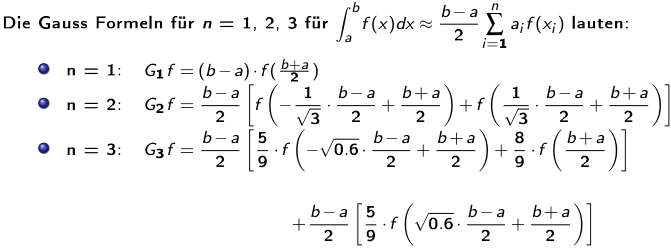
\includegraphics[scale=0.38]{int-gaussformeln}






\subsection{Romberg-Extrapolation}
% TODO code

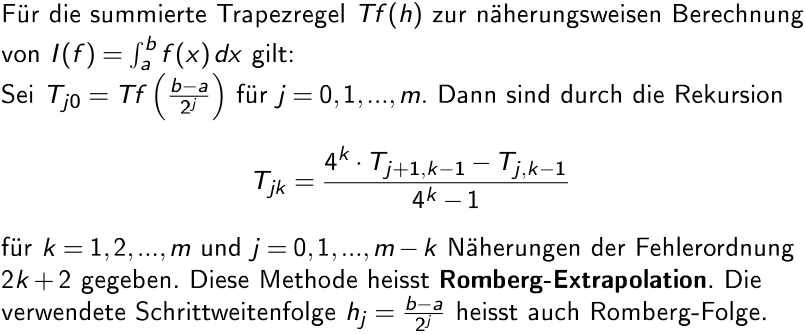
\includegraphics[scale=0.32]{int-romberg-extrapolation}

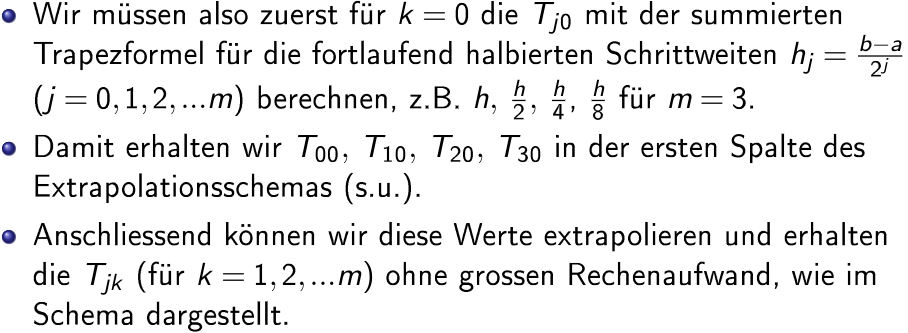
\includegraphics[scale=0.29]{int-romberg-extrapolation-2}

{\Large Die Extrapolation ergibt folgendes Schema ($m = 3$)}\\
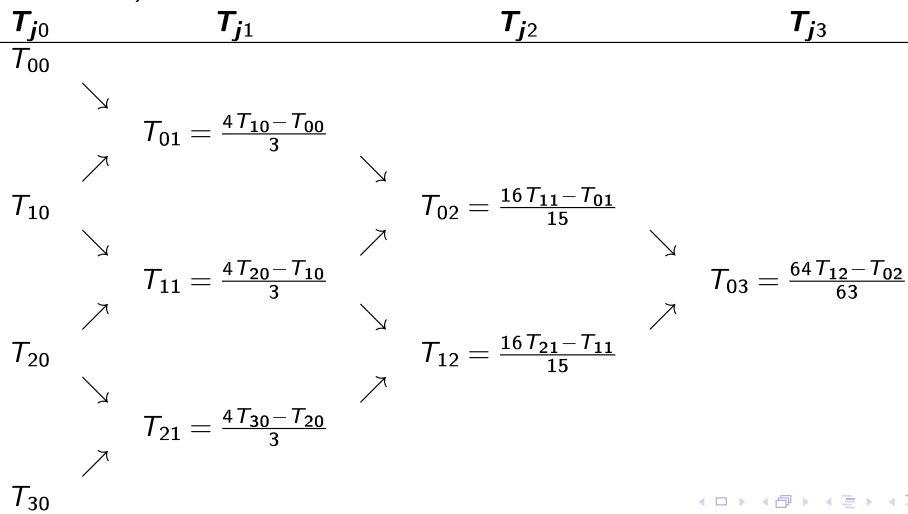
\includegraphics[scale=0.29]{int-romberg-extrapolation-schema}


\subsubsection{Bemerkungen zur Romberg-Extrapolation}

\begin{itemize}
	\item In der ersten Spalte $T_{j0}$ muss für die summierte Trapezregel Aufgrund
	      von $h_j = \frac{b-a}{2^j}$ natürlich auch $n_j = 2^j$ verwenden
	\item Da in der ersten Spalte $T_{j0}$ die Trapezeregel für immer kleiner
	      werdende Schrittweiten $h_j$ angewandt wird, werden oft unnötig $f(x_i)$
	      doppelt ausgewertet. Statdessen kann man diese spalte auch rekursiv definieren.
          $$T_{j0} = \frac{1}{2} T_{j-1,0} + h_{j-1}
            \sum_{i=1}^{n_{j-1}} f(a + (2i-1)h_{j-1})$$
          $$\text{wobei: } \quad n_{j-1} = 2^{j-1} \quad \& \quad h_{j-1} = \frac{h_{j-1}}{2}$$
\end{itemize}



